\documentclass[12pt]{article}
\usepackage[left=2cm, top=2cm, right=2cm, bottom=2cm]{geometry}
\usepackage[utf8]{inputenc}      % accents dans le source
\usepackage[T1]{fontenc}
\usepackage[french]{babel}
\usepackage{graphicx}
\usepackage{graphics}
\usepackage{amsmath}
\usepackage{amsfonts}
\usepackage{amssymb}
\usepackage{tikz}
\usepackage{xcolor} 
\usepackage{mathtools}
\usepackage{parskip}
\usepackage{subcaption}
\usepackage[export]{adjustbox}
\usepackage{hyperref}

\tikzset{every picture/.style={line width=0.75pt}}
\newcommand{\sinc}{\operatorname{sinc}}


\title{\textbf{Optique ondulatoire:} Diffraction de la lumière}
\author{MENARD Alexandre - VIEILLEDENT Florent}

\setlength{\parindent}{1cm}

\begin{document}
\maketitle

\section*{Introduction}

\break
\section{Diffraction par des ouvertures simples}
Dans cette première partie, nous nous intéressons au cas de la diffraction dans le cas d'ouvertures simples. Nous y proposerons une description qualitative, quantitative dans le cas d'une fente simple,
une description de motifs de diffraction pour différentes ouvertures. Enfin, nous proposerons un protocole permettant de déterminer avec précision le diamètre d'un cheveu en s'appuyant sur le théorème de Babinet.
\subsection{Etude d'une fente simple de largeur variable}
Pour une première approche, nous installons un laser face à un écran, et l'on insère une fente simple de largeur variable $a$ entre le laser et l'écran, à un distance $D$ de l'écran.
\begin{figure}[!h]
    \begin{center}
        \resizebox{0.7\textwidth}{5cm}{
        \begin{tikzpicture}[x=0.75pt,y=0.75pt,yscale=-1,xscale=1]
%uncomment if require: \path (0,300); %set diagram left start at 0, and has height of 300

%Flowchart: Process [id:dp872954957901976] 
\draw   (104,140) -- (184,140) -- (184,160) -- (104,160) -- cycle ;
%Straight Lines [id:da9241077852973352] 
\draw [color={rgb, 255:red, 208; green, 2; blue, 27 }  ,draw opacity=1 ][line width=0.75]    (184,150) -- (354,150) ;
\draw [shift={(275,150)}, rotate = 180] [color={rgb, 255:red, 208; green, 2; blue, 27 }  ,draw opacity=1 ][line width=0.75]    (10.93,-3.29) .. controls (6.95,-1.4) and (3.31,-0.3) .. (0,0) .. controls (3.31,0.3) and (6.95,1.4) .. (10.93,3.29)   ;
%Straight Lines [id:da39324764499965714] 
\draw    (354,160) -- (354,200) ;
%Straight Lines [id:da3239950960426152] 
\draw    (354,100) -- (354,140) ;
%Straight Lines [id:da8041456916959207] 
\draw [color={rgb, 255:red, 208; green, 2; blue, 27 }  ,draw opacity=1 ]   (354,150) -- (534,130) ;
\draw [shift={(449.96,139.34)}, rotate = 173.66] [color={rgb, 255:red, 208; green, 2; blue, 27 }  ,draw opacity=1 ][line width=0.75]    (10.93,-3.29) .. controls (6.95,-1.4) and (3.31,-0.3) .. (0,0) .. controls (3.31,0.3) and (6.95,1.4) .. (10.93,3.29)   ;
%Straight Lines [id:da7837201764569335] 
\draw [color={rgb, 255:red, 208; green, 2; blue, 27 }  ,draw opacity=1 ]   (354,150) -- (534,170) ;
\draw [shift={(449.96,160.66)}, rotate = 186.34] [color={rgb, 255:red, 208; green, 2; blue, 27 }  ,draw opacity=1 ][line width=0.75]    (10.93,-3.29) .. controls (6.95,-1.4) and (3.31,-0.3) .. (0,0) .. controls (3.31,0.3) and (6.95,1.4) .. (10.93,3.29)   ;
%Straight Lines [id:da08364499364029099] 
\draw  [dash pattern={on 0.84pt off 2.51pt}]  (354,150) -- (534,150) ;
%Straight Lines [id:da3720582141386004] 
\draw    (534,100) -- (534,200) ;
%Straight Lines [id:da4573530253324263] 
\draw    (366,240) -- (522,240) ;
\draw [shift={(524,240)}, rotate = 180] [color={rgb, 255:red, 0; green, 0; blue, 0 }  ][line width=0.75]    (10.93,-3.29) .. controls (6.95,-1.4) and (3.31,-0.3) .. (0,0) .. controls (3.31,0.3) and (6.95,1.4) .. (10.93,3.29)   ;
\draw [shift={(364,240)}, rotate = 0] [color={rgb, 255:red, 0; green, 0; blue, 0 }  ][line width=0.75]    (10.93,-3.29) .. controls (6.95,-1.4) and (3.31,-0.3) .. (0,0) .. controls (3.31,0.3) and (6.95,1.4) .. (10.93,3.29)   ;
%Straight Lines [id:da5804934197531184] 
\draw    (554,132) -- (554,168) ;
\draw [shift={(554,170)}, rotate = 270] [color={rgb, 255:red, 0; green, 0; blue, 0 }  ][line width=0.75]    (10.93,-3.29) .. controls (6.95,-1.4) and (3.31,-0.3) .. (0,0) .. controls (3.31,0.3) and (6.95,1.4) .. (10.93,3.29)   ;
\draw [shift={(554,130)}, rotate = 90] [color={rgb, 255:red, 0; green, 0; blue, 0 }  ][line width=0.75]    (10.93,-3.29) .. controls (6.95,-1.4) and (3.31,-0.3) .. (0,0) .. controls (3.31,0.3) and (6.95,1.4) .. (10.93,3.29)   ;

% Text Node
\draw (125,142) node [anchor=north west][inner sep=0.75pt]   [align=left] {Laser};
% Text Node
\draw (305,49) node [anchor=north west][inner sep=0.75pt]   [align=left] {Fente simple\\de largeur $\displaystyle a$};
% Text Node
\draw (438,212.4) node [anchor=north west][inner sep=0.75pt]    {$D$};
% Text Node
\draw (565,142.4) node [anchor=north west][inner sep=0.75pt]    {$L$};
% Text Node
\draw (515,62) node [anchor=north west][inner sep=0.75pt]   [align=left] {Ecran};


\end{tikzpicture}

        }
    \end{center}
    \caption{Schéma du montage}
\end{figure}

Pour une largeur fixe, nous observons une figure de diffraction avec une large tâche centrale, puis des zéros d'intensité et de nouvelles tâches qui se répetent de chaque côté de la tâche centrale.
En augmentant la largeur de la fente $a$, nous observons un resserement des tâches d'intensité maximale et lorsque l'on réduit la largeur, ces mêmes tâches s'élargissent.

% TODO: Insérer nos propres images des figures de diffraction dans ces parties ! Il faut penser à prendre nos photos
\begin{figure}[h!]
    \centering
    \begin{subfigure}{.33\textwidth}
      \centering
        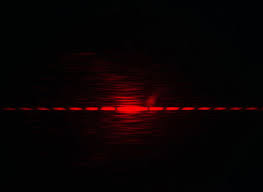
\includegraphics[width=.9\linewidth]{img/a_remplacer_par_nos_images.jpg}
      \caption{Largeur $a$ qui diminue}
      \label{fig:sfig1}
    \end{subfigure}%
    \begin{subfigure}{.33\textwidth}
      \centering
      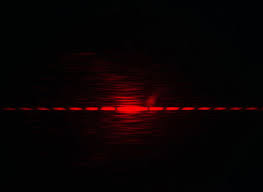
\includegraphics[width=.9\linewidth]{img/a_remplacer_par_nos_images.jpg}
      \caption{Largeur $a$ initiale}
      \label{fig:sfig2}
    \end{subfigure}
    \begin{subfigure}{.33\textwidth}
        \centering
        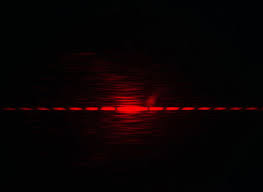
\includegraphics[width=.9\linewidth]{img/a_remplacer_par_nos_images.jpg}
        \caption{Largeur $a$ qui augmente}
        \label{fig:sfig3}
      \end{subfigure}
    \caption{Figure de diffraction en fonction de la largeur de la fente}
    \label{fig:fig}
\end{figure}

\break
Nous proposons ensuite de vérifier la formule qui donne la largeur de la tâche centrale $L$ pour des configurations différentes de $\lambda, D$ et $a$. Pour cela, nous devons
connaître les valeurs d'annulation de l'intensité en fonction de $y$.
\begin{align*}
    I(\theta) = I_0 \sinc^2\left(\frac{\pi a \sin \theta}{\lambda}\right) = 0 & \Leftrightarrow \sinc\left(\frac{\pi a \sin \theta}{\lambda}\right) = 0 \\
    & \Leftrightarrow \frac{\pi a \sin \theta}{\lambda} = n\pi, \forall n \in \mathbb{Z}^* \\
    & \Leftrightarrow \sin \theta = \frac{n\lambda}{a}
\end{align*}

Dans le cadre où $\theta$ très petit, on a $\theta \approx \sin \theta \approx \tan \theta $ et $\tan \theta = \frac{y}{D}$, il vient que:
\begin{align}
    \label{eqn:loi_intensite}
    y_n = \frac{n\lambda D}{a}, \forall n \in \mathbb{Z}^*
\end{align}

On peut alors en déduire la largeur $L$ de la tâche centrale qui s'étend entre les deux premiers minimums $n=1$ et $n=-1$ d'où:
\begin{align}
    L = \left\lvert y_{-1} - y_1 \right\rvert = \frac{2\lambda D}{a}
\end{align}

Pour vérifier cette loi (\ref{eqn:loi_intensite}), nous allons utiliser un seul et même montage, mais nous ferons varier un paramètre à la fois à savoir la longueur d'onde $\lambda$, la distance entre la fente et l'écran $D$, 
et la largeur de la fente $a$. Pour cela, nous plaçons un laser de longueur d'onde $\lambda$ face à un écran, et une fente de largeur $a$ entre les deux à une distance $D$ de l'écran.

\begin{figure}[!h]
    \begin{center}
        \resizebox{0.7\textwidth}{5cm}{
        

\begin{tikzpicture}[x=0.75pt,y=0.75pt,yscale=-1,xscale=1]
%uncomment if require: \path (0,300); %set diagram left start at 0, and has height of 300

%Flowchart: Process [id:dp872954957901976] 
\draw   (104,140) -- (184,140) -- (184,160) -- (104,160) -- cycle ;
%Straight Lines [id:da9241077852973352] 
\draw [color={rgb, 255:red, 208; green, 2; blue, 27 }  ,draw opacity=1 ][line width=0.75]    (184,150) -- (354,150) ;
\draw [shift={(275,150)}, rotate = 180] [color={rgb, 255:red, 208; green, 2; blue, 27 }  ,draw opacity=1 ][line width=0.75]    (10.93,-3.29) .. controls (6.95,-1.4) and (3.31,-0.3) .. (0,0) .. controls (3.31,0.3) and (6.95,1.4) .. (10.93,3.29)   ;
%Straight Lines [id:da39324764499965714] 
\draw    (354,160) -- (354,200) ;
%Straight Lines [id:da3239950960426152] 
\draw    (354,100) -- (354,140) ;
%Straight Lines [id:da8041456916959207] 
\draw [color={rgb, 255:red, 208; green, 2; blue, 27 }  ,draw opacity=1 ]   (354,150) -- (534,130) ;
\draw [shift={(449.96,139.34)}, rotate = 173.66] [color={rgb, 255:red, 208; green, 2; blue, 27 }  ,draw opacity=1 ][line width=0.75]    (10.93,-3.29) .. controls (6.95,-1.4) and (3.31,-0.3) .. (0,0) .. controls (3.31,0.3) and (6.95,1.4) .. (10.93,3.29)   ;
%Straight Lines [id:da7837201764569335] 
\draw [color={rgb, 255:red, 208; green, 2; blue, 27 }  ,draw opacity=1 ]   (354,150) -- (534,170) ;
\draw [shift={(449.96,160.66)}, rotate = 186.34] [color={rgb, 255:red, 208; green, 2; blue, 27 }  ,draw opacity=1 ][line width=0.75]    (10.93,-3.29) .. controls (6.95,-1.4) and (3.31,-0.3) .. (0,0) .. controls (3.31,0.3) and (6.95,1.4) .. (10.93,3.29)   ;
%Straight Lines [id:da08364499364029099] 
\draw  [dash pattern={on 0.84pt off 2.51pt}]  (354,150) -- (534,150) ;
%Straight Lines [id:da3720582141386004] 
\draw    (534,100) -- (534,200) ;
%Straight Lines [id:da4573530253324263] 
\draw    (366,240) -- (522,240) ;
\draw [shift={(524,240)}, rotate = 180] [color={rgb, 255:red, 0; green, 0; blue, 0 }  ][line width=0.75]    (10.93,-3.29) .. controls (6.95,-1.4) and (3.31,-0.3) .. (0,0) .. controls (3.31,0.3) and (6.95,1.4) .. (10.93,3.29)   ;
\draw [shift={(364,240)}, rotate = 0] [color={rgb, 255:red, 0; green, 0; blue, 0 }  ][line width=0.75]    (10.93,-3.29) .. controls (6.95,-1.4) and (3.31,-0.3) .. (0,0) .. controls (3.31,0.3) and (6.95,1.4) .. (10.93,3.29)   ;
%Straight Lines [id:da5804934197531184] 
\draw    (554,132) -- (554,168) ;
\draw [shift={(554,170)}, rotate = 270] [color={rgb, 255:red, 0; green, 0; blue, 0 }  ][line width=0.75]    (10.93,-3.29) .. controls (6.95,-1.4) and (3.31,-0.3) .. (0,0) .. controls (3.31,0.3) and (6.95,1.4) .. (10.93,3.29)   ;
\draw [shift={(554,130)}, rotate = 90] [color={rgb, 255:red, 0; green, 0; blue, 0 }  ][line width=0.75]    (10.93,-3.29) .. controls (6.95,-1.4) and (3.31,-0.3) .. (0,0) .. controls (3.31,0.3) and (6.95,1.4) .. (10.93,3.29)   ;

% Text Node
\draw (118,140) node [anchor=north west][inner sep=0.75pt]   [align=left] {Laser $\displaystyle \lambda $};
% Text Node
\draw (305,49) node [anchor=north west][inner sep=0.75pt]   [align=left] {Fente simple\\de largeur $\displaystyle a$};
% Text Node
\draw (438,212.4) node [anchor=north west][inner sep=0.75pt]    {$D$};
% Text Node
\draw (565,142.4) node [anchor=north west][inner sep=0.75pt]    {$L$};
% Text Node
\draw (515,62) node [anchor=north west][inner sep=0.75pt]   [align=left] {Ecran};


\end{tikzpicture}

        }
    \end{center}
    \caption{Schéma du montage}
\end{figure}

\subsubsection{Influence de la largeur de la fente}
Pour ce premier paramètre, nous allons placer différentes fentes de largeur $a$ calibrée à une distance $D = \dots cm$ de l'écran, et l'on illumine les différentes fentes avec un laser de longueur d'onde
$\lambda = \dots nm$. 

\subsubsection{Influence de la longueur d'onde}
Pour ce second paramètre, nous fixons une fente de largeur $a = \dots \mu m$ calibrée, à une distance $D = \dots cm$ de l'écran, et l'on placera différents laser de longueur d'onde $\lambda$.

\subsubsection{Influence de la distance entre l'écran et la fente}
Pour ce dernier paramètre, nous illuminons une fente de largeur $a = \dots \mu m$ calibrée, avec un laser de longueur d'onde $\lambda = \dots nm$ et nous allons faire varier la distance $D$ entre la fente et l'écran.

\subsubsection{Synthèse et analyse des résultats expérimentaux}

\break
\subsection{Caractérisation de la figure de diffraction par une fente simple avec une caméra linéaire}

\subsection{Etude de différents motifs de diffraction}

\break
\subsection{Théorème de Babinet et taille d'un cheveu}
Le théorème de Babinet donne que la figure de diffraction d'un objet et de son complémentaire est la même.
Ainsi, un fil et une fente de même épaisseur $a$ forment dont une seule et même figure d'interférence ayant la même largeur de tâche centrale. Cette propriété permet la mesure de longueur très petite, que nous allons utiliser
pour déterminer le diamètre d'un cheveu.

On commence par positionner un laser de longueur d'onde $\lambda = \dots nm$ face à un écran. A l'aide du jeton A3015 que l'on place à une distance $D = \dots cm$ de
l'écran, on mesure la largeur de la tâche centrale $L_a$ pour chaque largeur de fente $a$. Enfin, on place à cette même distance $D$ le cheveu dont on souhaite déterminer
le diamètre et l'on mesure la largeur de la tâche centrale $L_{cheveu}$. On peut ensuite comparer $L_{cheveu}$ pour trouver une correspondance dans les différents $L_a$ précédent, et si l'on a une 
correspondance, nous pouvons conclure que l'épaisseur $d_{cheveu} \approx a$.

\begin{figure}[!h]
    \begin{center}
        \resizebox{0.7\textwidth}{8cm}{
        \begin{tikzpicture}[x=0.75pt,y=0.75pt,yscale=-1,xscale=1]
    %uncomment if require: \path (0,429); %set diagram left start at 0, and has height of 429

    %Flowchart: Process [id:dp7587016517098488] 
    \draw   (110,120) -- (190,120) -- (190,140) -- (110,140) -- cycle ;
    %Straight Lines [id:da1423603054270386] 
    \draw [color={rgb, 255:red, 208; green, 2; blue, 27 }  ,draw opacity=1 ][line width=0.75]    (190,130) -- (360,130) ;
    \draw [shift={(281,130)}, rotate = 180] [color={rgb, 255:red, 208; green, 2; blue, 27 }  ,draw opacity=1 ][line width=0.75]    (10.93,-3.29) .. controls (6.95,-1.4) and (3.31,-0.3) .. (0,0) .. controls (3.31,0.3) and (6.95,1.4) .. (10.93,3.29)   ;
    %Straight Lines [id:da16631230033992783] 
    \draw    (360,140) -- (360,180) ;
    %Straight Lines [id:da6025420297783186] 
    \draw    (360,80) -- (360,120) ;
    %Straight Lines [id:da364809732100976] 
    \draw [color={rgb, 255:red, 208; green, 2; blue, 27 }  ,draw opacity=1 ]   (360,130) -- (540,110) ;
    \draw [shift={(455.96,119.34)}, rotate = 173.66] [color={rgb, 255:red, 208; green, 2; blue, 27 }  ,draw opacity=1 ][line width=0.75]    (10.93,-3.29) .. controls (6.95,-1.4) and (3.31,-0.3) .. (0,0) .. controls (3.31,0.3) and (6.95,1.4) .. (10.93,3.29)   ;
    %Straight Lines [id:da29487712829226687] 
    \draw [color={rgb, 255:red, 208; green, 2; blue, 27 }  ,draw opacity=1 ]   (360,130) -- (540,150) ;
    \draw [shift={(455.96,140.66)}, rotate = 186.34] [color={rgb, 255:red, 208; green, 2; blue, 27 }  ,draw opacity=1 ][line width=0.75]    (10.93,-3.29) .. controls (6.95,-1.4) and (3.31,-0.3) .. (0,0) .. controls (3.31,0.3) and (6.95,1.4) .. (10.93,3.29)   ;
    %Straight Lines [id:da5859877642355407] 
    \draw  [dash pattern={on 0.84pt off 2.51pt}]  (360,130) -- (540,130) ;
    %Straight Lines [id:da8840842764785435] 
    \draw    (540,80) -- (540,180) ;
    %Straight Lines [id:da5130608383839474] 
    \draw    (372,220) -- (528,220) ;
    \draw [shift={(530,220)}, rotate = 180] [color={rgb, 255:red, 0; green, 0; blue, 0 }  ][line width=0.75]    (10.93,-3.29) .. controls (6.95,-1.4) and (3.31,-0.3) .. (0,0) .. controls (3.31,0.3) and (6.95,1.4) .. (10.93,3.29)   ;
    \draw [shift={(370,220)}, rotate = 0] [color={rgb, 255:red, 0; green, 0; blue, 0 }  ][line width=0.75]    (10.93,-3.29) .. controls (6.95,-1.4) and (3.31,-0.3) .. (0,0) .. controls (3.31,0.3) and (6.95,1.4) .. (10.93,3.29)   ;
    %Straight Lines [id:da9345083369474423] 
    \draw    (560,112) -- (560,148) ;
    \draw [shift={(560,150)}, rotate = 270] [color={rgb, 255:red, 0; green, 0; blue, 0 }  ][line width=0.75]    (10.93,-3.29) .. controls (6.95,-1.4) and (3.31,-0.3) .. (0,0) .. controls (3.31,0.3) and (6.95,1.4) .. (10.93,3.29)   ;
    \draw [shift={(560,110)}, rotate = 90] [color={rgb, 255:red, 0; green, 0; blue, 0 }  ][line width=0.75]    (10.93,-3.29) .. controls (6.95,-1.4) and (3.31,-0.3) .. (0,0) .. controls (3.31,0.3) and (6.95,1.4) .. (10.93,3.29)   ;
    %Flowchart: Process [id:dp0037548894552708045] 
    \draw   (110,280) -- (190,280) -- (190,300) -- (110,300) -- cycle ;
    %Straight Lines [id:da6846741364957676] 
    \draw [color={rgb, 255:red, 208; green, 2; blue, 27 }  ,draw opacity=1 ][line width=0.75]    (190,290) -- (360,290) ;
    \draw [shift={(281,290)}, rotate = 180] [color={rgb, 255:red, 208; green, 2; blue, 27 }  ,draw opacity=1 ][line width=0.75]    (10.93,-3.29) .. controls (6.95,-1.4) and (3.31,-0.3) .. (0,0) .. controls (3.31,0.3) and (6.95,1.4) .. (10.93,3.29)   ;
    %Straight Lines [id:da021706815786682876] 
    \draw [color={rgb, 255:red, 208; green, 2; blue, 27 }  ,draw opacity=1 ]   (360,290) -- (540,270) ;
    \draw [shift={(455.96,279.34)}, rotate = 173.66] [color={rgb, 255:red, 208; green, 2; blue, 27 }  ,draw opacity=1 ][line width=0.75]    (10.93,-3.29) .. controls (6.95,-1.4) and (3.31,-0.3) .. (0,0) .. controls (3.31,0.3) and (6.95,1.4) .. (10.93,3.29)   ;
    %Straight Lines [id:da044428076418244755] 
    \draw [color={rgb, 255:red, 208; green, 2; blue, 27 }  ,draw opacity=1 ]   (360,290) -- (540,310) ;
    \draw [shift={(455.96,300.66)}, rotate = 186.34] [color={rgb, 255:red, 208; green, 2; blue, 27 }  ,draw opacity=1 ][line width=0.75]    (10.93,-3.29) .. controls (6.95,-1.4) and (3.31,-0.3) .. (0,0) .. controls (3.31,0.3) and (6.95,1.4) .. (10.93,3.29)   ;
    %Straight Lines [id:da4536520815231391] 
    \draw  [dash pattern={on 0.84pt off 2.51pt}]  (360,290) -- (540,290) ;
    %Straight Lines [id:da2719763791486136] 
    \draw    (540,240) -- (540,340) ;
    %Straight Lines [id:da9223524271493639] 
    \draw    (560,272) -- (560,308) ;
    \draw [shift={(560,310)}, rotate = 270] [color={rgb, 255:red, 0; green, 0; blue, 0 }  ][line width=0.75]    (10.93,-3.29) .. controls (6.95,-1.4) and (3.31,-0.3) .. (0,0) .. controls (3.31,0.3) and (6.95,1.4) .. (10.93,3.29)   ;
    \draw [shift={(560,270)}, rotate = 90] [color={rgb, 255:red, 0; green, 0; blue, 0 }  ][line width=0.75]    (10.93,-3.29) .. controls (6.95,-1.4) and (3.31,-0.3) .. (0,0) .. controls (3.31,0.3) and (6.95,1.4) .. (10.93,3.29)   ;
    %Shape: Circle [id:dp9133941073673402] 
    \draw  [fill={rgb, 255:red, 0; green, 0; blue, 0 }  ,fill opacity=1 ] (355,290) .. controls (355,287.24) and (357.24,285) .. (360,285) .. controls (362.76,285) and (365,287.24) .. (365,290) .. controls (365,292.76) and (362.76,295) .. (360,295) .. controls (357.24,295) and (355,292.76) .. (355,290) -- cycle ;
    %Straight Lines [id:da8477820676507002] 
    \draw    (360,340) -- (360,302) ;
    \draw [shift={(360,300)}, rotate = 90] [color={rgb, 255:red, 0; green, 0; blue, 0 }  ][line width=0.75]    (10.93,-3.29) .. controls (6.95,-1.4) and (3.31,-0.3) .. (0,0) .. controls (3.31,0.3) and (6.95,1.4) .. (10.93,3.29)   ;

    % Text Node
    \draw (131,122) node [anchor=north west][inner sep=0.75pt]   [align=left] {Laser};
    % Text Node
    \draw (311,29) node [anchor=north west][inner sep=0.75pt]   [align=left] {Fente simple\\de largeur $\displaystyle a$};
    % Text Node
    \draw (518,361) node [anchor=north west][inner sep=0.75pt]   [align=left] {Ecran};
    % Text Node
    \draw (444,192.4) node [anchor=north west][inner sep=0.75pt]    {$D$};
    % Text Node
    \draw (571,122.4) node [anchor=north west][inner sep=0.75pt]    {$L_{a}$};
    % Text Node
    \draw (131,282) node [anchor=north west][inner sep=0.75pt]   [align=left] {Laser};
    % Text Node
    \draw (292,349) node [anchor=north west][inner sep=0.75pt]   [align=left] {Cheveu de diamètre\\$\displaystyle d_{cheveu}$ à déterminer};
    % Text Node
    \draw (571,282.4) node [anchor=north west][inner sep=0.75pt]    {$L_{cheveu}$};
    % Text Node
    \draw (521,42) node [anchor=north west][inner sep=0.75pt]   [align=left] {Ecran};
\end{tikzpicture}
        }
    \end{center}
    \caption{Schéma du protocole}
\end{figure}

Cependant, il est possible que les fentes disponibles dans le jeu A3015 ne soient pas suffisantes pour avoir une valeur précise. Pour résoudre ce problème, nous pouvons
simplement mesurer les distances $y_n$ où la figure de diffraction présente des zéros d'intensités, et d'utiliser la formule suivante donnant les $y_n$ d'intensité nulle:
\begin{align}
    y_n = \frac{n\lambda D}{d_{cheveu}}
\end{align}

On peut donc remonter à $d_{cheveu}$ en déterminant le coefficient directeur $y(n) = \frac{D}{d_{cheveu}} n$ de nos mesures expérimentales.



\newpage

\section*{Annexes}
\subsection{Démonstration sans approximation des petits angles}
Nous avons $\sin \theta = \frac{y}{\sqrt{D^2+y^2}}$ ce qui nous donne alors:
\begin{align*}
    \sin \theta = \frac{n\lambda}{a} & \Leftrightarrow \frac{y}{\sqrt{D^2+y^2}} = \frac{n\lambda}{a} \\
    & \Leftrightarrow a^2y^2 = n^2 \lambda ^2 \left( D^2 + y^2 \right) \\
    & \Leftrightarrow y^2 = \frac{n^2 \lambda^2 D^2}{a^2 - n^2 \lambda^2} \\
    & \Leftrightarrow y = \pm \frac{n \lambda D}{\sqrt{a^2 - n^2 \lambda^2}}
\end{align*}

Enfin, dans l'approximation où $\lambda \ll a$, nous avons :
\begin{align}
    y = \pm \frac{n \lambda D}{a}
\end{align}

On retrouve bien l'approximation des petits angles.

\end{document}
